% =================================================================================================
% File:			nome_del_documento.tex
% Description:	Defiinisce la struttura del documento di Nome del documento 
% Created:		2015-01-29
% Author:		Tesser Paolo
% Email:		p.tesser921@gmail.com
% =================================================================================================
% Modification History:
% Version		Modifier Date		Change											Author
% 0.0.1 		2015-01-29 			stesura documento di prova						Tesser Paolo
% =================================================================================================
%

% TEMPLATE DA USARE AD OGNI NUOVO DOCUMENTO

% =================================================================================================
% File:			package.tex
% Description:	Defiinisce i pacchetti utilizzati per generare i documenti
% Created:		2014-12-05
% Author:		Santacatterina Luca
% Email:		s88.luca@gmail.com
% =================================================================================================
% Modification History:
% Version		Modifier Date		Change												Author
% 0.0.1 		2014-12-05 			Prima emissione 									Luca S.
% =================================================================================================
% 0.0.2			2014-12-17			cambio colori per i link in black					Tesser Paolo
% =================================================================================================
% 0.0.3			2014-12-23			inserito package caption e settato valore skip a 1	Tesser Paolo
% =================================================================================================
% 0.0.4			2015-01-15			aggiunto package per grafici a barre				Tesser Paolo

\documentclass[11pt,a4paper]{article}
\usepackage[left=3.5cm,right=3.5cm,top=3.0cm,bottom=2.5cm]{geometry}
\usepackage[font=small,labelfont=bf]{caption}
\usepackage[italian]{babel}
\usepackage[utf8]{inputenc}
\usepackage[T1]{fontenc}

\usepackage{color}
\usepackage{enumitem}
\usepackage{eurosym}
\usepackage{fancyhdr}
\usepackage{geometry}
\usepackage{graphicx}
\usepackage{hyperref}
\usepackage{lastpage}
\usepackage{lastpage}
\usepackage{listings}
\usepackage{longtable}
\usepackage{multirow}
\usepackage{pdflscape}
\usepackage{pdfpages}
\usepackage{subcaption}
\usepackage{tabularx}
\usepackage{tikz}
\usepackage{pgfkeys}
\usepackage{titlesec}
\usepackage{verbatim}
\usepackage{xr}
\usepackage{xspace}
\usepackage[skip=1pt]{caption} % package che gestisce lo spazione tra la figura e la sua caption
\usepackage{sectsty}
\usepackage{pgfplots}

\pagestyle{fancy}

\hypersetup{
	colorlinks=true,
	linkcolor=black,
	urlcolor=blue
}

\setcounter{secnumdepth}{5}
\setcounter{tocdepth}{5}

% =================================================================================================
% File:			commands.tex
% Description:	Defiinisce i comandi personalizzati utilizzati per redarre i documenti
% Created:		2014-12-05
% Author:		Santacatterina Luca
% Email:		s88.luca@gmail.com
% =================================================================================================
% Modification History:
% Version		Modifier Date		Change												Author
% 0.0.1 		2014-12-05 			Prima emissione 									Luca S.
% =================================================================================================
% 0.0.2 		2014-12-13 			Inseriti comandi nome e la vers. dei file 			Luca S.
% =================================================================================================
% 0.0.3			2014-12-19			inserito comando per richiamare il libro di testo	Tesser Paolo
% =================================================================================================
% 0.0.4			2015-01-02			inserito comando per le revisioni					Tesser Paolo
% =================================================================================================
% 0.0.5			2015-01-07			inseriti comandi per i documenti mancanti			Tesser Paolo
% =================================================================================================
% 0.0.6			2015-01-12			cambiata versione dei documenti a 1.0.0				Tesser Paolo
% =================================================================================================
% 0.0.7			2015-01-14			comandi per la generazione di grafici a torta/barre	Tesser Paolo

% DEFINIZIONE COMANDI BASE CHE POI ANDRANNO RIDEFINITI

% ==================================================================================================
% COMANDI DA RIDEFINIRE
% ==================================================================================================

% Nome/Versione/Data del documento
\newcommand{\documentName}{ERRORE}
\newcommand{\documentVersion}{ERRORE}
\newcommand{\documentDate}{ERRORE}

% Editori del documento
\newcommand{\documentEditors}{ERRORE}

% Verificatore del documento
\newcommand{\documentVerifiers}{ERRORE}

% Approvazione del documento
\newcommand{\documentApprovers}{ERRORE}

% Lista di distribuzione del documento
\newcommand{\documentDistributionList}{\groupName\\\commitNameM\\\commitNameS\\\proposerName}

% Uso del documento
\newcommand{\documentUsage}{ERRORE}

% Sommario del documento
\newcommand{\documentSummary}{ERRORE}

% Vesione dei documenti
\newcommand{\docVersionAdR}{\emph{v1.0.0}} % Analisi dei Requisiti
\newcommand{\docVersionGlo}{\emph{v1.0.0}} % Glossario
\newcommand{\docVersionNdP}{\emph{v1.0.0}} % Norme di Progetto
\newcommand{\docVersionPdP}{\emph{v1.0.0}} % Piano di Progetto
\newcommand{\docVersionPdQ}{\emph{v1.0.0}} % Piano di Qualifica
\newcommand{\docVersionSdF}{\emph{v1.0.0}} % Studio di Fattibilità
\newcommand{\docVersionST}{\emph{v1.0.0}} % Specifica Tecnica
\newcommand{\docVersionDdP}{\emph{v1.0.0}} % Definizione di Prodotto
\newcommand{\docVersionMU}{\emph{v1.0.0}} % Manuale Utente

% ==================================================================================================
% COMANDI DA NON RIDEFINIRE
% ==================================================================================================

% Nome del progetto
\newcommand{\projectName}{BDSMApp}
\newcommand{\groupEmail}{\textit{\href{mailto:info@mashup-unipd.it}{info@mashup-unipd.it}}}
\newcommand{\groupName}{\emph{MashUp}}

% Ruoli del progetto
\newcommand{\roleProjectManager}{\emph{Responsabile di Progetto}}
\newcommand{\roleAdministrator}{\emph{Amministratore di Progetto}}
\newcommand{\roleAnalyst}{\emph{Analista}}
\newcommand{\roleProgrammer}{\emph{Programmatore}}
\newcommand{\roleDesigner}{\emph{Progettista}}
\newcommand{\roleVerifier}{\emph{Verificatore}}

% Referenti e commitenti (M = master, S = slave)
\newcommand{\proposerName}{\emph{Dott. David Santucci} - Zing Srl}
\newcommand{\commitNameM}{\emph{Prof. Tullio Vardanega}}
\newcommand{\commitNameS}{\emph{Prof. Riccardo Cardin}}

% Abbreviazioni per richiamare il nome esteso dei diversi documenti da redarre
\newcommand{\docGlossary}{\emph{Glossario}} 
\newcommand{\docAdR}{\emph{Analisi dei Requisiti \currentVersion}}
\newcommand{\docNdP}{\emph{Norme di Progetto \currentVersion}}
\newcommand{\docPdP}{\emph{Piano di Progetto \currentVersion}}
\newcommand{\docPdQ}{\emph{Piano di Qualifica \currentVersion}}
\newcommand{\docSdF}{\emph{Studio di Fattibilità \currentVersion}}

% Nome dei documenti
\newcommand{\docNameAdR}{\emph{Analisi dei Requisiti}} % Analisi dei Requisiti
\newcommand{\docNameGlo}{\emph{Glossario}} % Glossario
\newcommand{\docNameNdP}{\emph{Norme di Progetto}} % Norme di Progetto
\newcommand{\docNamePdP}{\emph{Piano di Progetto}} % Piano di Progetto
\newcommand{\docNamePdQ}{\emph{Piano di Qualifica}} % Piano di Qualifica
\newcommand{\docNameSdF}{\emph{Studio di Fattibilità}} % Studio di Fattibilità
\newcommand{\docNameST}{\emph{Specifica Tecnica}} % Specifica Tecnica
\newcommand{\docNameDdP}{\emph{Definizione di Prodotto}} % Definizione di Prodotto
\newcommand{\docNameMU}{\emph{Manuale Utente}} % Manuale Utente

% Nome e versione dei documenti
\newcommand{\docNameVersionAdR}{\docNameAdR{} \docVersionAdR} % Analisi dei Requisiti
\newcommand{\docNameVersionGlo}{\docNameGlo{} \docVersionGlo} % Glossario
\newcommand{\docNameVersionNdP}{\docNameNdP{} \docVersionNdP} % Norme di Progetto
\newcommand{\docNameVersionPdP}{\docNamePdP{} \docVersionPdP} % Piano di Progetto
\newcommand{\docNameVersionPdQ}{\docNamePdQ{} \docVersionPdQ} % Piano di Qualifica
\newcommand{\docNameVersionSdF}{\docNameSdF{} \docVersionSdF} % Studio di Fattibilità
\newcommand{\docNameVersionST}{\docNameST{} \docVersionST} % Specifica Tecnica
\newcommand{\docNameVersionDdP}{\docNameDdP{} \docVersionDdP} % Definizione di Prodotto
\newcommand{\docNameVersionMU}{\docNameMU{} \docVersionMU} % Manuale Utente

% Nome delle revisioni
\newcommand{\RR}{\emph{Revisione dei Requisiti}}
\newcommand{\RPmin}{\emph{Revisione di Progettazione minima}}
\newcommand{\RPmax}{\emph{Revisione di Progettazione massima}}
\newcommand{\RQ}{\emph{Revisione di Qualifica}}
\newcommand{\RA}{\emph{Revisione di Accettazione}}

% Descrizione scopo del glossario
\newcommand{\glossarioDesc}{Al fine di evitare ogni ambiguità relativa al linguaggio usato nei documenti viene allegato il \docNameVersionGlo.
Esso ha lo scopo di definire ed analizzare tutti i termini tecnici del progetto e di fugare eventuali ambiguità fornendo un'accurata descrizione.\\
Tutte le occorrenze di tali termini nei documenti verranno contrassegnate con una ``G'' a pedice.}

% Descrizione dello scopo del prodtto
\newcommand{\productScope}{Lo scopo del prodotto è di creare una nuova infrastruttura che permetta di interrogare Big Data recuperati dai social network, quali: Facebook, Twitter, Instagram.
L'applicazione sarà composta da due parti:
	\begin{itemize}
		\item consultazione e interrogazione con interfaccia web per utente;
		\item servizi web REST interrogabili.
	\end{itemize}
}

\newcommand{\sommerville}{Software Engineering - Ian Sommerville - 9th Edition(2010)}

% Comandi per la generazione di grafici a torta e a barre
\newcommand{\pie}[3][]{
    \begin{scope}[#1]
    \pgfmathsetmacro{\curA}{90}
    \pgfmathsetmacro{\r}{1}
    \def\c{(0,0)}
    \node[pie title] at (90:1.3) {#2};
    \foreach \v\s in{#3}{
        \pgfmathsetmacro{\deltaA}{\v/100*360}
        \pgfmathsetmacro{\nextA}{\curA + \deltaA}
        \pgfmathsetmacro{\midA}{(\curA+\nextA)/2}

        \path[slice,\s] \c
            -- +(\curA:\r)
            arc (\curA:\nextA:\r)
            -- cycle;
        \pgfmathsetmacro{\d}{max((\deltaA * -(.5/50) + 1) , .5)}

        \begin{pgfonlayer}{foreground}
        \path \c -- node[pos=\d,pie values,values of \s]{$\v\%$} +(\midA:\r);
        \end{pgfonlayer}

        \global\let\curA\nextA
    }
    \end{scope}
}

\newcommand{\legend}[2][]{
    \begin{scope}[#1]
    \path
        \foreach \n/\s in {#2}
            {
                  ++(0,-5pt) node[\s,legend box] {} +(5pt,0) node[legend label] {\n} % ++(x,y) -> y: spazio tra i vari campi della legenda, x: l'obliquità
            }
    ;
    \end{scope}
}

% Comandi per il glossario
\newcommand{\gloss}{\ped{\textbf{\tiny G}}}

% Comando per abbassare versione PDF
\pdfminorversion=4
% =================================================================================================
% File:			package.tex
% Description:	Defiinisce  lo stile che viene utilizzato nelle pagine dei documenti
% Created:		2015-01-29
% Author:		Tesser Paolo
% Email:		p.tesser921@gmail.com
% =================================================================================================
% Modification History:
% Version		Modifier Date		Change											Author
% 0.0.1 		2015-01-29 			Prima emissione 								Tesser Paolo
% =================================================================================================
%

\fancypagestyle{styleFirstPage}{

}


\fancypagestyle{styleIndexPage}{	
	\pagestyle{empty}
	% HEADER
	\fancyhead{}
	\setlength{\topmargin}{-65pt}
	\setlength{\headsep}{65pt}
	\fancyhfoffset[L]{\marginparwidth - \marginparsep}
	\fancyhfoffset[R]{\marginparwidth - \marginparsep}
	\fancyhead[L]{\definecolor{titlepagecolor}{cmyk}{0,0,0,0.20}
	\begin{tikzpicture}[remember picture,overlay]
		\path [fill=titlepagecolor](-20,1.8) rectangle(1\paperwidth,-0.3);
	\end{tikzpicture}
	
\includegraphics[width=150pt]{../template/images/logo/logo_orizzontale.pdf}}
	\fancyhead[R]{\uppercase{\leftmark}}
	% FOOTER
	\fancyfoot[L]{}
	\fancyfoot[R]{}
	\fancyfoot[C]{\thepage}
	\pagenumbering{Roman}
	\renewcommand{\footrulewidth}{0.0pt}
	\renewcommand{\headrulewidth}{0.0pt}
}


\fancypagestyle{styleDocPages}{
	\thispagestyle{empty}
	\thispagestyle{fancy}
	\pagestyle{fancy}
	% HEADER
	\fancyhead{}
	\setlength{\topmargin}{-65pt}
	\setlength{\headsep}{65pt}
	\fancyhfoffset[L]{\marginparwidth - \marginparsep}
	\fancyhfoffset[R]{\marginparwidth - \marginparsep}
	\fancyhead[L]{\definecolor{titlepagecolor}{cmyk}{0,0,0,0.20}
	\begin{tikzpicture}[remember picture,overlay]
		\path [fill=titlepagecolor](-20,1.8) rectangle(1\paperwidth,-0.3);
	\end{tikzpicture}
	
\includegraphics[width=150pt]{../template/images/logo/logo_orizzontale.pdf}}
	\fancyhead[R]{\uppercase{\leftmark}}
	% FOOTER
	\fancyfoot{}
	\fancyfoot[L]{\documentName~\documentVersion}
	\fancyfoot[R]{Pagina \thepage~di~\pageref{LastPage}}
	\setcounter{page}{0}
	\pagenumbering{arabic}
	\renewcommand{\headrulewidth}{0.0pt}
  	\renewcommand{\footrulewidth}{0.2pt}
}

% Definizione stile e forme per grafici a torta e a barre
\definecolor{rosso}{RGB}{220,57,18} % per ruolo di an
\definecolor{giallo}{RGB}{255,153,0} % per ruolo di pt
\definecolor{blu}{RGB}{102,140,217} % per ruolo di pm
\definecolor{verde}{RGB}{16,150,24} % per ruolo di pr
\definecolor{viola}{RGB}{127,245,212} % per ruolo di am (non è viola)
\definecolor{rame}{RGB}{184,115,51} % per ruolo di ve

\makeatletter

\tikzstyle{chart}=[
    legend label/.style={font={\scriptsize},anchor=west,align=left},
    legend box/.style={rectangle, draw, minimum size=7pt},
    axis/.style={black,semithick,->},
    axis label/.style={anchor=east,font={\normalsize}},
]

\tikzstyle{bar chart}=[
    chart,
    bar width/.code={
        \pgfmathparse{##1/2}
        \global\let\bar@w\pgfmathresult
    },
    bar/.style={very thick, draw=white},
    bar label/.style={font={\bf\small},anchor=north},
    bar value/.style={font={\footnotesize}},
    bar width=.75,
]

\tikzstyle{pie chart}=[
    chart,
    slice/.style={line cap=round, line join=round, very thick,draw=white},
    pie title/.style={font={\bf}},
    slice type/.style 2 args={
        ##1/.style={fill=##2},
        values of ##1/.style={}
    }
]

\pgfdeclarelayer{background}
\pgfdeclarelayer{foreground}
\pgfsetlayers{background,main,foreground}

\begin{document}
	% COMANDI DA RIDEFINIRE
	\renewcommand{\documentName}{Guida a Git}
	\renewcommand{\documentVersion}{v.1.0.0}
	\renewcommand{\documentDate}{2015-01-29}
	\renewcommand{\documentEditors}{Tesser Paolo}
	% \renewcommand{\documentVerifiers}{Cognome Nome\\Cognome Nome}
	% \renewcommand{\documentApprovers}{Cognome Nome\\Cognome Nome}
	% \renewcommand{\documentUsage}{Esterno}
	\renewcommand{\documentSummary}{Questa guida serve per raccogliere i comandi più utilizzati in git e le best practice per applicarli}

	% FRONTESPIZIO
	\pagenumbering{gobble}
	\pagestyle{styleFirstPage}
	% =================================================================================================
% File:			firstpage.tex
% Description:	Defiinisce i contenuti obbligatori della prima pagina
% Created:		2015-01-29
% Author:		Tesser Paolo
% Email:		p.tesser921@gmail.com
% =================================================================================================
% Modification History:
% Version		Modifier Date		Change											Author
% 0.0.1 		2015-01-29 			Prima emissione 								Tesser Paolo
% =================================================================================================
%

% DEFINIZIONE DELLA PRIMA PAGINA

\thispagestyle{empty}
\setlength{\topmargin}{70pt}
% NOME DELLA GUIDA
\begin{center}
	\Large \textbf{NOME DELLA GUIDA}
\end{center}

% SE SI VUOLE ANCHE IL LOGO (DA AGGIUNGERE NEW COMMAND CON L'INCLUDE DINAMICO)
\begin{comment}
	\begin{figure}[!t]
		\centering
		
\includegraphics[width=10cm]{../template/images/logo/zing.pdf}
	\end{figure}
\end{comment}


% Informazioni del documento
\begin{center}
\vspace{1.5cm}
	\textbf{\Large Informazioni Documento} \\[1pt]
	\begin{longtable}{|l|p{180pt}|}
		\hline
		\textbf{Nome documento} & \documentName \\
		\hline
		\textbf{Versione} & \documentVersion \\
		\hline
		\textbf{Data redazione} & \documentDate \\
		\hline
		\textbf{Redattori} & \parbox[t]{\textwidth}{\documentEditors} \\
		\hline
		% \textbf{Verificatori} & \parbox{\textwidth}{\documentVerifiers} \\ & \\
		% \textbf{Approvazione} & \parbox{\textwidth}{\documentApprovers} \\ & \\
		% \textbf{Lista distribuzione} & \parbox{\textwidth}{\documentDistributionList} \\ & \\
		\textbf{Uso} & \parbox{\textwidth}{\documentUsage} \\
		\hline
	\end{longtable}
	\vspace{20pt}
		\textbf{\Large Sommario} \\
		\documentSummary
\end{center}

	\pagebreak


	% PAGINA REVISIONI & PAGINA INDICI
	\setcounter{page}{1}
	\pagestyle{styleIndexPage}
	% =================================================================================================
% File:			history.tex
% Description:	Defiinisce le modifiche effettuate nel documento
% Created:		2015-01-29
% Author:		Tesser Paolo
% Email:		p.tesser921@gmail.com
% =================================================================================================
% Modification History:
% Version		Modifier Date		Change											Author
% 0.0.1 		2015-01-29 			inserite due history di prova 					Tesser Paolo
% =================================================================================================
%

\begin{center}
\begin{small}
	\textbf{\huge Diario Revisioni}
	\vspace{0.5cm}
	\begin{longtable}{|p{6cm}|c|c|c|}
		\hline
		\textbf{Modifica} & \textbf{Autore} & \textbf{Data} & \textbf{Versione} \\
		\hline
		Stesura parte sulle configurazioni & Tesser Paolo & 2015-02-02 & v0.0.2 \\
		\hline
		Inizio stesura del documento & Tesser Paolo & 2015-01-29 & v0.0.1 \\
		\hline
	\end{longtable}

\end{small}
\end{center}\pagebreak
	\tableofcontents \pagebreak
	% \listoftables \pagebreak
	\listoffigures \pagebreak

	% PAGINE CONTENUTI
	\setcounter{page}{1}
	\pagestyle{styleDocPages}
	% =================================================================================================
% File:			content_files.tex
% Description:	Defiinisce i capitoli presenti nel documento
% Created:		2015-01-29
% Author:		Tesser Paolo
% Email:		p.tesser921@gmail.com
% =================================================================================================
% Modification History:
% Version		Modifier Date		Change											Author
% 0.0.1 		2015-01-29 			inserito capitolo di prova						Tesser Paolo
% =================================================================================================
%

% DEFINIZIONE DEI CONTENUTI DEL DOCUMENTO

% =================================================================================================
% File:			all.tex
% Description:	Defiinisce la sezione relativa a ...
% Created:		2015-01-29
% Author:		Tesser Paolo
% Email:		p.tesser921@gmail.com
% =================================================================================================
% Modification History:
% Version		Modifier Date		Change											Author
% 0.0.1 		2015-01-29 			iniziata stesura documento di prova				Tesser Paolo
% =================================================================================================
% 0.0.2			2015-02-02			aggiunta img + migliorata sez. configurazioni	Tesser Paolo
% =================================================================================================
% 0.0.3			2015-02-02			aggiunta sezione per i workflow, da stendere	Tesser Paolo
% =================================================================================================
%


% CONTENUTO DEL CAPITOLO

\section{Introduzione} % (fold)
\label{sec:introduzione}
Git è un sistema di controllo di versione distribuito. \\
\textbf{Distribuito} (DVCS) significa che ogni componente, del gruppo di lavoro, possiede una copia locale completa del repository. \\

\noindent
\textbf{Vantaggi}:
	\begin{itemize}
		\item operazioni di commit più veloci da effettuare;
		\item si riesce a lavorare offline;
		\item ognuno ha in locale un backup del repository.
	\end{itemize}
	\noindent
	\\
La seguente immagine serve per dare un idea generale di come git lavori e tramite quali operazioni di base. Viene mostrato inoltre il rapporto tra la gestione in locale del repository con quello in remoto. Il dettaglio delle operazioni sarà illustrato prevalentemente nella sezione \ref{sec:lavorare_sul_repository}.

	\begin{figure}[htbp]
		\centering
		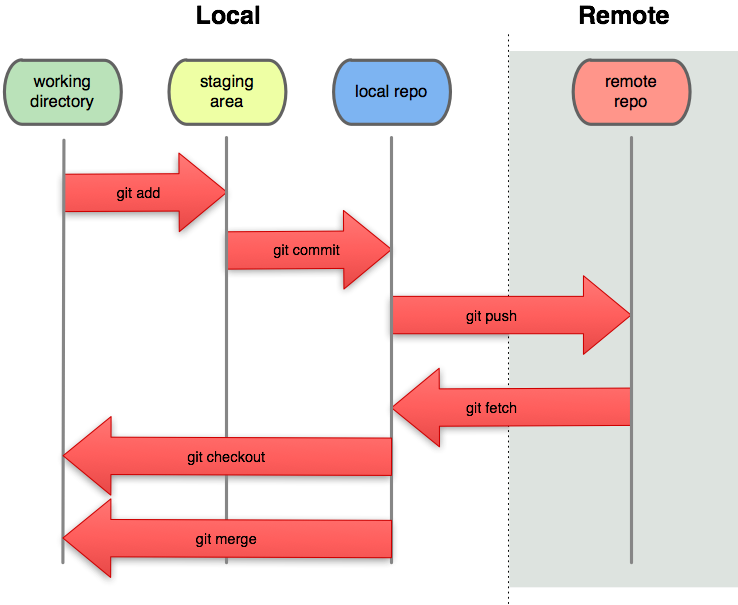
\includegraphics[scale=1.1]{images/git_local_remote.png}
		\caption{Git - Locale e Remoto}
		\label{fig:git_locale_e_remoto}
	\end{figure}


	\subsection{Informativi} % (fold)
	\label{sub:informativi}
		\begin{itemize}
			\item \textbf{CodeSchool}: \url{www.codeschool.com};
			\item \textbf{CERN - Best Practice}: PDF;
		\end{itemize}
	% subsection informativi (end)

% section introduzione (end)

\newpage \clearpage
\section{Riferimenti} % (fold)
\label{sec:riferimenti}
Di seguito viene spiegato attraverso quali nomi git si riferisce a determinati stati del versionamento. \\ \\

\textbf{Riferimenti specifici}:
	\begin{itemize}
		\item \textbf{Working Tree}: è l'insieme di file su cui si sta lavorando non ancora aggiunti alla staging area (vedi sezione \ref{sub:lavorare_in_locale});
		\item \textbf{Index}: è il riferimento ai file pronti per essere committati, quelli aggiunti alla staging area;
		\item \textbf{HEAD}: è il riferimento all'ultimo commit effettuato;
		\item \textbf{d3a7c852d2c789f791b11091894cc71387e562e9}: un valore hash attribuito ad ogni commit;
		\item \textbf{master, feature-eg}: il nome esatto di un branch per riferirsi ad esso;
		\item \textbf{v1.0.0}: il nome di un tag per riferirsi ad esso.
	\end{itemize}
	\noindent
\textbf{Riferimenti relativi}:
\begin{comment}
	\begin{itemize}
		\item il commit precedente: ref\textasciitilde1 oppure ref^;
		\item il penultimo commit: ref\textasciitilde2 oppure ref^^;
		\item genitori differenti: ref^1. (TO LEARN).
	\end{itemize}
\end{comment}

% section riferimenti (end)


\newpage \clearpage
\section{Impostare git} % (fold)
\label{sec:impostare_git}
La prima volta che si installa git è buona pratica impostare da subito alcune credenziali. \\
Queste credenziali possono essere impostate su diversi livelli:
	\begin{itemize}
		\item \textbf{global}: valide quindi per tutti i repository dell'utente. Si trovano nel file:
			\begin{center}
				~/.gitconfig
			\end{center}
		\item \textbf{system}: valide per tutti i repository del computer. Si trovano nel file:
			\begin{center}
				/etc/gitconfig
			\end{center}
		\item \textbf{local}: valide solo per il repository dal quale vengono impostate. Si trovano nel file:
			\begin{center}
				.git/config
			\end{center}
	\end{itemize}
Da linea di comando eseguire i seguenti comandi, cambiando l'opzione ``global'' a seconda delle esigenze:
	\begin{verbatim}
	path: git config --global user.name "Nome Cognome"
	path: git config --global user.email mail@mail.com
	path: git config --global color.ui true
	path: git config --global core.editor emacs
	path: git config --global commit.template ~/.gitmessage.txt
	\end{verbatim}

% section impostare_git (end)

\newpage \clearpage
\section{Creare un repository} % (fold)
\label{sec:creare_un_repository}
Un repository può essere creato in locale e usato solo nel computer dell'utente, anche se questo non permetterà un lavoro collaborativo, oppure, dopo la creazione in locale, può essere associato ad un repository creato su un server (o attraverso un servizio di hosting). \\
Per creare un repository su un servizio di hosting basta seguire le istruzione che il sito propone.
	\subsection{Creazione in locale} % (fold)
	\label{sub:creazione_in_locale}
	Di seguito viene illustrata la sequenza di comandi che dovranno essere eseguiti:
		\begin{verbatim}
		path: mkdir nome_repo
		path: cd nome_repo
		path: git init
		\end{verbatim}
	\noindent
	L'ultima istruzione creerà tutti i metadati necessari al repository. Verranno salvati nella cartella nascosta:
		\begin{center}
			nome\_repo/.git/
		\end{center}

	% subsection creazione_in_locale (end)
	
% section creare_un_repository (end)

\newpage \clearpage
\section{Lavorare sul repository} % (fold)
\label{sec:lavorare_sul_repository}

	\subsection{Lavorare in locale} % (fold)
	\label{sub:lavorare_in_locale}
	Le tre azioni che vengono più spesso eseguite quando si lavora in locale sono:
		\begin{itemize}
			\item creare un file;
			\item aggiungerlo alla \textbf{staging area} attraverso il comando:
				\begin{verbatim}
				path: git add nome_del_file.ext
				\end{verbatim}
				\noindent
				La staging area è il luogo dove sono presenti i file pronti per essere committati.
				Se si vogliono aggiungere più file contemporaneamente o solo alcuni, possiamo eseguire in esclusione questi comandi:
					\begin{verbatim}
					path: git add --all # aggiunge tutti i file presenti nella unstaging area
					path: git add <list of file>
					path: git add *.ext
					path: git add dir/
					\end{verbatim}
				\noindent
				\textbf{Buona pratica}, come verrà illustrato di seguito, vuole che i commit siano il più possibile atomici. \'E \textbf{consigliato fortemente} quindi eseguire il comando:
					\begin{verbatim}
					path: git add --patch (o -p)
					\end{verbatim}
				\noindent
				Questo comando permettere di revisionare il codice che si sta aggiungendo, con la possibilità di scartarne delle parti;

			\item committare i cambiamenti attraverso il comando:
				\begin{verbatim}
				path: git commit -m "msg"
				\end{verbatim}
				\noindent
				Quest'ultima operazione può essere effettuata anche senza l'opzione -m, in tal caso la procedura seguirà lo schema illustrato nella sezione TO DO; \\
				Importante e \textbf{obbligatorio} è effettuare commit atomici in quanto se qualcosa andasse storto, per colpa di qualche inserimento sbagliato, sarebbe più facile effettuare una ricerca dell'errore. Inoltre, questa metodologia, permette di dare una descrizione più efficace sul messaggio di cosa si sta facendo e soprattutto meno prolissa in quanto vado ad aggiungere meno cose contemporaneamente. \\
				Il messaggio che viene inserito deve essere di facile interpretazione. Non bisogna scrivere cose generiche o superflue.
				 
		\end{itemize}
	\noindent
	Per osservare i cambiamenti avvenuti dall'ultima operazione di commit basta lanciare il comando:
		\begin{verbatim}
		path: git status
		\end{verbatim}

	
		\subsubsection{Visualizzare le differenze} % (fold)
		\label{ssub:visualizzare_le_differenze}
		Per osservare le differenze di un file in relazione a dove si trova:
			\begin{verbatim}
			# per osservare le modifiche sui file non ancora inseriti nella staging area con quelli presenti su Index
			path: git diff nome_del_file
			# per osservare le modifiche sui file già inseriti nella staging area con quelli presenti su HEAD
			path: git diff --staged nome_del_file
			# per osservare le modifiche sui file nella staging area rispetto a quelli su HEAD
			path: git diff HEAD
			\end{verbatim}

		% subsubsection visualizzare_le_differenze (end)
		
		\subsubsection{Rimuovere i file dalla staging area} % (fold)
		\label{ssub:rimuovere_i_file_dalla_staging_area}
		Per rimuovere dei file aggiunti nella staging area, tramite il comando \textbf{git add}, bisogna lanciare il seguente comando:
			\begin{verbatim}
			path: git reset HEAD # per rimuovere tutti i file
			path: git reset HEAD nome_del_file # per rimuovere solo quello specificato
			\end{verbatim}
		\noindent
		La variabile Index viene portata indietro di un passo. \\ \\
		Per annullare l'ultimo commit dobbiamo eseguire il seguente comando:
			\begin{verbatim}
			path: git reset --soft HEAD^
			\end{verbatim}
		\noindent
		L'opzione --\textbf{soft} serve a lasciare i file, dell'ultima commit, nella staging area, quindi puntati dalla variabile Index. \\
		La direttiva \textbf{HEAD\^} serve per annullare i commit solo fino al penultimo, cioè quello precedente di quello che vogliano annullare. \\
		La variabile HEAD viene portata indietro di un passo. \\
		\textbf{Nota}: questi comandi non annullano le modifiche effettuate ai file. \\

		Per rimuovere l'ultimo commit dobbiamo eseguire il seguente comando:
			\begin{verbatim}
			path: git reset --hard HEAD^
			\end{verbatim}
		\noindent
		Le variabili HEAD, Index e Working Tree vengono portate indietro di un passo. \\
		Questo comando è potenzialmente dannoso perché rischi di farti perdere il lavoro presente nella Working Tree. \'E bene quindi utilizzarlo solo quando il comando \textbf{git status} dia un output pulito. \\
		Non bisogna inoltre usare questo comando quando il commit è stato pushato in un repository pubblico, perché altri sviluppatori potrebbero fare riferimento ad un istanza che verrebbe rimossa.
		
 		% subsubsection rimuovere_i_file_dalla_staging_area (end)
		
		\subsubsection{Annullare i cambiamenti} % (fold)
		\label{ssub:annullare_i_cambiamenti}
		Per riportare i file che si sono modificati, ma non ancora committati, allo stato dell'ultimo commit, bisogna eseguire il seguente comando:
			\begin{verbatim}
			path: git checkout -- nome_del_file
			\end{verbatim}
		% subsubsection annullare_i_cambiamenti (end)

		\subsubsection{Ripristinare precedenti versioni} % (fold)
		\label{ssub:ripristinare_precedenti_versioni}
		TO DO
		% subsubsection ripristinare_precedenti_versioni (end)


		\subsubsection{Branch} % (fold)
		\label{ssub:branch}
		A differenza di altri sistemi di versionamento, in git un branch è semplicemente un puntatore a un commit. \\
		Le operazioni di branching sono elencate di seguito:
			\begin{itemize}
				\item creare un branch:
					\begin{verbatim}
					path: git branch nome_del_branch [punto di partenza]
					\end{verbatim}
				\item cancellare un branch:
					\begin{verbatim}
					path: git branch -d|-D nome_del_branch
					\end{verbatim}
				\item muoversi tra i diversi branch:
					\begin{verbatim}
					path: git checkout nome_del_branch_dove_spostarsi
					\end{verbatim}
				Questo comando può essere eseguito solo quando non ci sono file ancora da committare;
				\item creare e spostarsi nel branch appena generato:
					\begin{verbatim}
					path: git checkout -b nome_del_branch
					\end{verbatim}
				\item rinominare un branch:
					\begin{verbatim}
					path: git branch -m nome_del_branch_vecchio nome_del_branch_nuovo
					\end{verbatim}
			\end{itemize}
			\noindent
		TO DO
		% subsubsection branch (end)


		\subsubsection{Tag} % (fold)
		\label{ssub:tag}
		TO DO
		% subsubsection tag (end)
		
	% subsection lavorare_in_locale (end)
	
	\subsection{Lavorare in remoto} % (fold)
	\label{sub:lavorare_in_remoto}
	TO DO
		\subsubsection{Pubblicare un branch} % (fold)
		\label{ssub:pubblicare_un_branch}
		TO DO
		% subsubsection pubblicare_un_branch (end)

		\subsubsection{Pubblicare un tag} % (fold)
		\label{ssub:pubblicare_un_tag}
		TO DO
		% subsubsection pubblicare_un_tag (end)

	% subsection lavorare_in_remoto (end)

% section lavorare_sul_repository (end)

\newpage \clearpage
\section{Git Hooks} % (fold)
\label{sec:git_hooks}
TO DO


% section git_hooks (end)




\newpage \clearpage
\section{Workflow} % (fold)
\label{sec:workflow}
In questa sezione vengono illustrati alcuni modelli di sviluppo che si possono adottare, principalmente nei lavori di gruppo, ma anche a livello personale. Ognuno di questi utilizzati git in diverse maniere a seconda delle sue caratteristiche.
	\subsection{Branching Model} % (fold)
	\label{sub:branching_model}
	In riferimento all'articolo presente al link: \\
	\url{http://nvie.com/posts/a-successful-git-branching-model/}, viene esposto il modello di sviluppo su git basato su diversi branch. \\
	TO DO
	\begin{figure}[htbp]
		\centering
		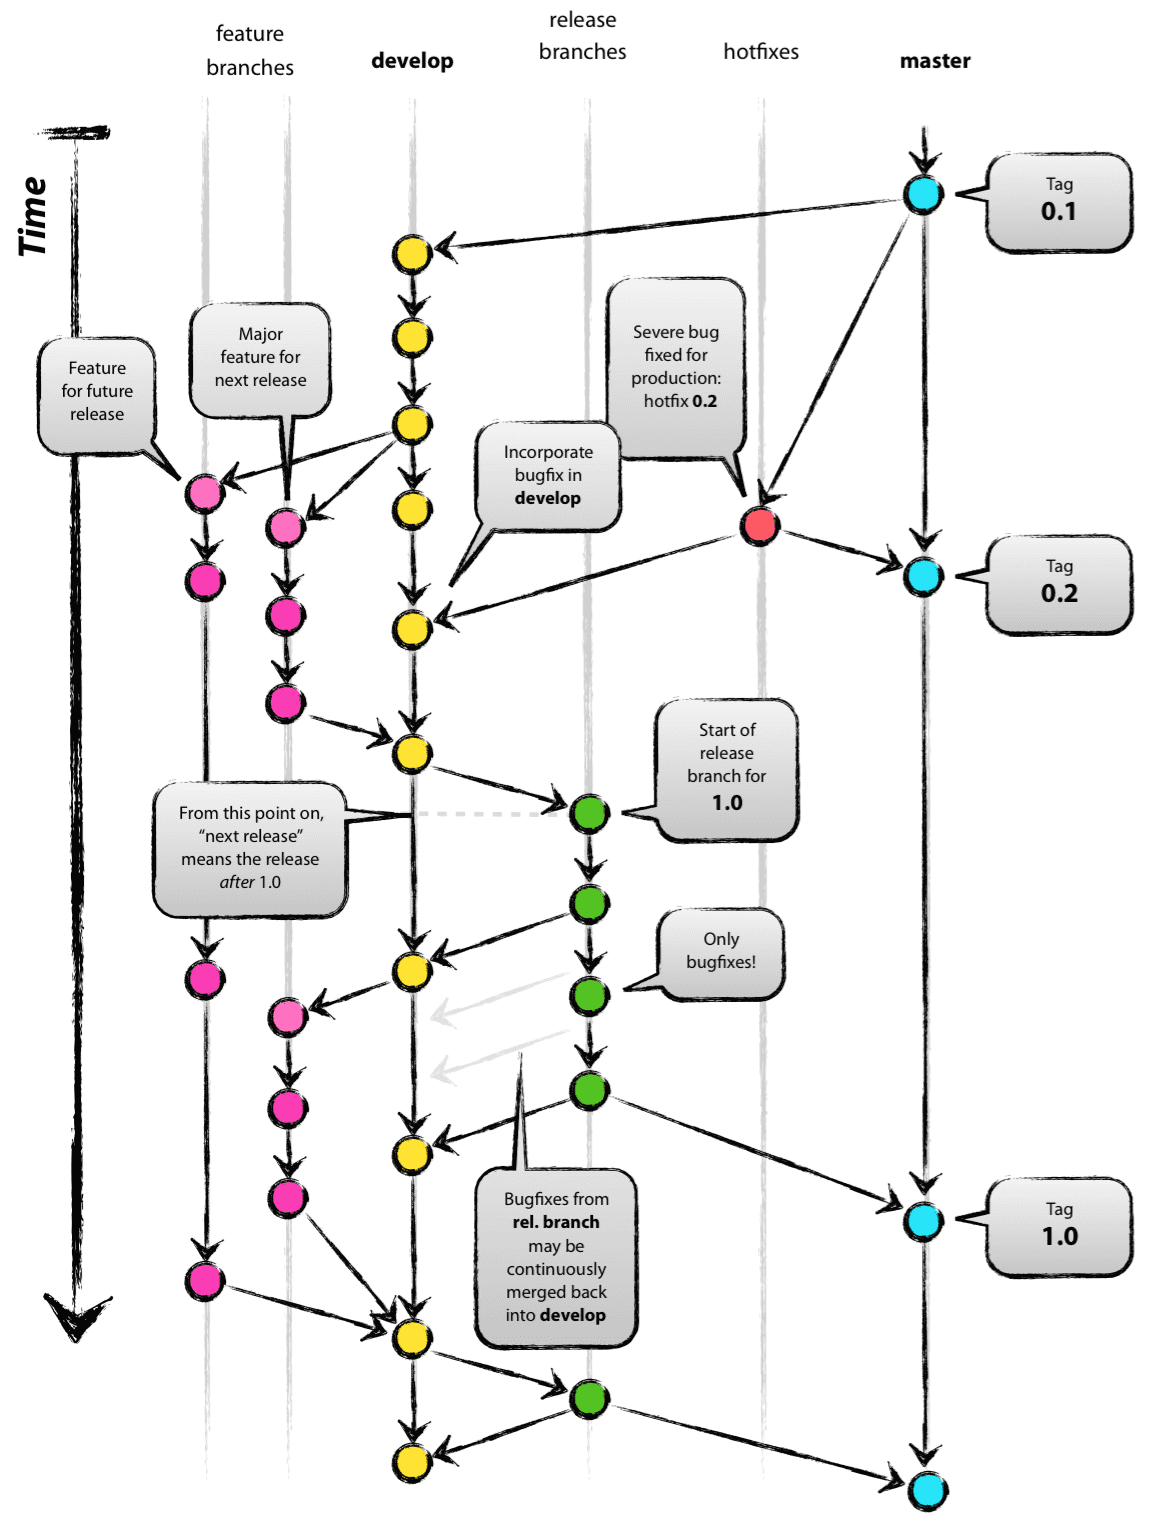
\includegraphics[scale=0.4]{images/git_branch_workflow.png}
		\caption{Git - Branch Workflow Model}
		\label{fig:git_branch_workflow_model}
	\end{figure}
	% subsection branching_model (end)
% section workflow (end)


\newpage \clearpage

\end{document}